\chapter{Wprowadzenie}
\label{cha:wprowadzenie}

%---------------------------------------------------------------------------

\section{Cel pracy}
\label{sec:cel}
Celem niniejszej pracy była rozbudowa biometrycznego systemu kotroli dostępu, identyfikującego lub weryfikującego tożsamość na podstawie tęczówki oka. Wśród głównych zadań znajdowała się budowa stanowiska do akwizycji obrazu tęczówki. Ponadto, należało poprawić istniejący algorytm mający na celu wydzielenie obszaru tęczówki, ekstrakcję jej cech oraz utworzenie kodu biometrycznego na ich podstawie. Wymagana była również rozbudowa istniejącej bazy danych i~wiążące się z~tym uzupełnienie interfejsu programu nowymi funkcjami. Tworzony program został oparty na systemie zaprezentowanym w pracy \cite{Gl11}.

W procesie tworzenia systemu oraz jego opisu, Tomasz Drzewiecki był odpowiedzialny za realizację modułu biometrycznego (\ref{cha:realizacja}) i~związanego z~nim opisu testów działania i~wniosków (rozdział \ref{cha:testywnioski}). Joanna Gajda odpowiadała za stworzenie bazy danych wraz z~rozszerzeniem interfejsu użytkownika, opisanych w rozdziale \ref{cha:systemKontroli}, a także teoretyczną charakterystykę biometrycznego systemu kontroli dostępu (\ref{cha:wprowadzenie}).

\section{Biometria oraz jej zastosowania w~historii i~współcześnie}
\label{sec:biometria}

Biometria jest, zgodnie z~definicjami zaczerpniętymi z~\cite{Ko75} oraz \cite{Bio01}, nauką obejmującą swoim zakresem badanie zmienności populacji organizmów. Wyniki tych badań, po opracowaniu z~uwzględnieniem szerokiego zakresu metod statystyki matematycznej, wykorzystywane są w~wielu różnych dziedzinach, między innymi antropologii, medycynie czy kryminalistyce. Z~punktu widzenia techniki, zadaniem biometrii jest dokonywanie pomiarów istot żywych, w~tym w~szczególności cech charakterystycznych ludzi, które pozwoliłoby na automatyczne rozpoznawanie i~weryfikację osób \cite{Bio01}\cite{Jain00}.

Identyfikacja biometryczna uwzględnia w~swoich metodach dwa rodzaje cech człowieka ~\cite{Bio01}\cite{Bio02}\cite{Jain00}\cite{Jain08}:
\begin{itemize} 
\item fizyczne - na przykład tęczówka lub siatkówka oka, linie papilarne palców dłoni, układ naczyń krwionośnych, kształt dłoni, kształt ucha, obraz twarzy oraz rozkład temperatur na niej, charakterystyka uzębienia, DNA, 
\item behawioralne - sposób poruszania się, dynamika podpisu, sposób pisania na klawiaturze komputera czy cechy charakterystyczne głosu.
\end{itemize}

Wśród tradycyjnych metod identyfikacji bądź weryfikacji tożsamości możemy wyróżnić \cite{Jain00}\cite{Jain08}:
\begin{itemize}
\item oparte na posiadanych tokenach (ang. \emph{token-based}), takich jak dowód tożsamości, paszport czy karta kredytowa,
\item oparte na posiadanej wiedzy (ang. \emph{knowledge-based}), czyli haśle, numerze PIN czy innym kodzie dostępu,
\end{itemize}
W~porównaniu z~tradycyjnymi sposobami rozpoznawania i~weryfikacji tożsamości, metody biometryczne okazują się być o~wiele skuteczniejszym rozwiązaniem. Jest to spowodowane dużym prawdopodobieństwem zawodności tradycyjnych metod w sytuacjach, gdy posiadany token zostanie zgubiony, ulegnie kradzieży bądź sfałszowaniu lub kod dostępu unikalny dla danego użytkownika zostaje przechwycony albo zapomniany. Tradycyjne sposoby identyfikacji i~weryfikacji nie gwarantują rozróżnienia pomiędzy właściwym posiadaczem danego tokenu lub wiedzy, a~osobą, która weszła w~posiadanie danych dostępowych w~sposób bezprawny. Metody biometryczne wychodzą naprzeciw temu wymaganiu ze względu na tworzenie wzorca charakteryzującego człowieka w oparciu o~informacje niesione przez unikalne dla niego cechy \cite{Jain00}. Ponadto, zwalniają one użytkownika z~obowiązku tworzenia, zapamiętywania i~przechowywania wiedzy lub przedmiotów koniecznych do identyfikacji/weryfikacji tożsamości \cite{Jain08}.  

Biometria miała zastosowanie już w~przeszłości, na przykład poprzez pobieranie odcisków palców w~celu potwierdzenia transakcji handlowych w~czasach starożytnych, czy w~trakcie rejestracji więźniów w~XIX wieku \cite{Bio02}\cite{HF1}. Współcześnie, jest to jedna z~najprężniej rozwijających się dziedzin bio- oraz teleinformatyki, której rozwiązania służą najczęściej jako forma kontroli dostępu i~autoryzacji tożsamości użytkowników określonych pomieszczeń, urządzeń, danych i~programów. Biometryczna identyfikacja tożsamości jest używana jako alternatywna, szybka i~efektywna forma odprawy paszportowej pasażerów na lotniskach i~granicach państwowych (poprzez analizowanie obszaru twarzy lub tęczówki oka) oraz do wyszukiwania osób w~bazie i~monitoringu czasu pracy w~firmach \cite{Bio01}\cite{Bio02}.

Metody identyfikacji biometrycznej różnią się, poza formą analizy oraz wariantem analizowanych cech, skutecznością poprawności rozpoznawania danej osoby na podstawie próbek danych opisujących jej cechy, wymaganym stopniem zaangażowania analizowanej osoby w~proces zbioru danych koniecznych do dokonania pomiarów oraz odpornością na oszustwa. Porównanie kilku metod biometrycznych zostało omówione w~\cite{Gl11}. Z~uwagi na dużą skuteczność i~względnie prostą mierzalność, w~niniejszej pracy skupiono się na identyfikacji w oparciu o~obraz tęczówki oka.


%---------------------------------------------------------------------------

\section{Charakterystyka identyfikacji biometrycznej na podstawie tęczówki oka}
\label{sec:zawartoscPracy}

Tęczówka ludzkiego oka jest jednym z~najbardziej charakterystycznych elementów twarzy człowieka, indywidualnym i~niepowtarzalnym ze względu na połączenie uwarunkowanego genetycznie koloru oraz złożonej struktury, wynikającej z~różnorodnych procesów fizycznych i~chemicznych, kształtujących ją w~pierwszych latach ludzkiego życia \cite{Iris01}\cite{Iris02}. Cechy te są wykorzystywane w~procesie biometrycznej identyfikacji jednostki, który opiera się na zastosowaniu różnorodnych matematycznych metod rozpoznawania wzorców w~algorytmach operujących na pobranym z~użyciem specjalistycznej kamery obrazie oka.

Pobranie stabilnego i~wolnego od zakłóceń obrazu ludzkiego oka wymaga pewnego stopnia współpracy ze strony osoby badanej, jednakże współczesne kamery i~sprzęt projektowane specjalnie do tego typu identyfikacji, są  coraz lepiej przystosowane do automatycznej akwizycji obrazu wysokiej rozdzielczości. ~W związku z~tym możliwe jest, iż z~upływem czasu będą one mogły operować bez bezpośredniej kooperacji ze strony badanego.

Współcześnie stosowane kamery, wykorzystywane w~celu akwizycji obrazu oka, operują we współpracy z~czujnikami działającymi w środowisku bliskiej podczerwieni (NIR, ang. \emph{Near-Infra Red}) lub obserwowalnej długości fali (VW, ang. \emph{Visible Wavelength}). Promieniowanie podczerwone efektywnie wspomaga pobieranie tego typu obrazów ze względu na kilka czynników:
\begin{itemize} 
\item w~zakresie widma NIR wyraźnie uwidaczniają się cechy posiadanej przez znaczną część populacji ludzkiej tęczówki w~odcieniach brązu,
\item promieniowanie to pomaga w~likwidowaniu powstałych na powierzchni oka odblasków światła z~otoczenia,
\item jest ono nieinwazyjne, w związku z~czym nieszkodliwe dla oka.
\end{itemize}
Natomiast technika \emph{Visible Wavelength} zachowuje informację na temat barwników przeważających w~budowie tęczówki, co umożliwia pozyskanie danych dotyczących charakterystycznych wzorców występujących na obrazie. Obie technologie mają swoje zalety i~wady; ich porównanie oraz próby połączenia w~celu uzyskania dokładniejszego sposobu pozyskiwania zdjęć tęczówki i~większej ilości niesionych wraz z~tym informacji zostały opisane w~pracy \cite{Hos10}. 

Proces identyfikacji na podstawie tęczówki, po uzyskaniu poprawnego obrazu przy pomocy kamery, dzieli się na kilka głównych etapów: \begin{itemize}
\item segmentacja, mająca na celu wyodrębnienie wewnętrznej i~zewnętrznej granicy tęczówki na obrazie oka, wraz z~szeregiem operacji, mających za zadanie wyeliminowanie zakłóceń na zdjęciu, w~postaci otaczających tęczówkę rzęs, powiek czy powstałych w~wyniku wpływu oświetlenia odblasków,
\item normalizacja, służąca do kompensacji deformacji tęczówki w~związku z~jej ewentualnym zwężeniem lub rozszerzeniem,
\item ekstrakcja cech tęczówki w~celu uzyskania unikalnego kodu, podlegającego późniejszej analizie z~zastosowaniem różnorodnych kryteriów, decydujących o~identyfikacji bądź pozytywnym lub negatywnym wyniku weryfikacji tożsamości danej osoby.
\end{itemize}

Schemat przedstawiający działanie typowego systemu identyfikacji biometrycznej na podstawie tęczówki oka znajduje się na diagramie ~\ref{fig:identyfikacja}. Został on utworzony w oparciu o~ogólne schematy działania typowych systemów identyfikacji biometrycznej, umieszczonych w ~\cite{Bio02} i~\cite{Jain00}.
\begin{figure}[b]
\begin{center}
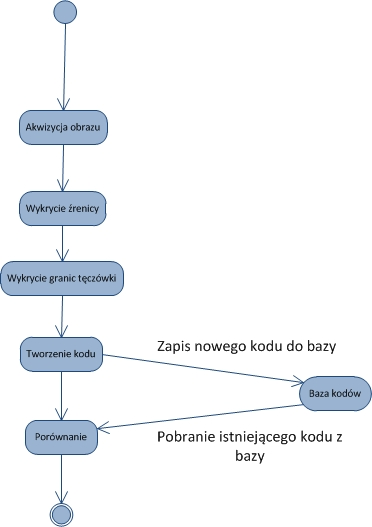
\includegraphics{schemat.jpg}
\caption{Schemat typowego systemu identyfikacji biometrycznej na podstawie tęczówki oka}
\label{fig:identyfikacja}
\end{center}
\end{figure}

Różnorodność metod segmentacji obszaru tęczówki oraz ekstrakcji cech i~porównywania kodów została opisana w~dalszych częściach pracy. Nie pokrywa ona oczywiście wszystkich metod obecnie znanych w~tej dziedzinie, jednakże w~niniejszej pracy starano się scharakteryzować jak największy ich podzbiór w~oparciu o~dostępną literaturę.


\section{Metody segmentacji obszaru tęczówki oka}
\label{sec:segmentacja}

Istnieje wiele metod segmentacji tęczówki \cite{PrAl06}. Pierwszą efektywnie zrealizowaną w~systemie biometrycznym metodę zaproponował John Daugman \cite{Daugman}. Rozwiązanie to, jak wiele innych, późniejszych, opiera się na założeniu, że źrenica oraz tęczówka stanowią okręgi. Stosuje się w~nim operator \ref{eq:daugman}.
\begin{equation}
\label{eq:daugman}
max_{r,x_{0},y_{0}}\left| G_{\sigma}(r) \frac{\delta}{\delta r}\int_{r,x_{0},y_{0}} \frac{i(x,y)}{2\pi r}ds \right|
\end{equation}
gdzie:\\
$ x,y $ - położenie piksela na obrazie, \\
$ x_{0}, y_{0} $ - położenie środka okręgu na obrazie, \\
$ r $ - promień okręgu, \\
$ ~I(x,y) $ - jasność piksela na obrazie,\\
$ G_{\sigma}(r) $ - rozkład Gaussa.

Dzięki temu można odnaleźć środek okręgu oraz jego promień, dla których będziemy mieli największą wartość pochodnej względem najbliższego otoczenia. Ta metoda jest skuteczna dla obrazów, gdzie wyraźna jest granica między źrenicą a~tęczówką oraz między tęczówką a~rogówką. Częste jest w~niej zastosowanie łuku dla szukania granicy między tęczówką a~rogówką, ponieważ zdarza się, że część tęczówki jest zakryta przez powieki \cite{Kr11}. Po skutecznie zrealizowanym algorytmie otrzymuje obraz podobny do przedstawionego na rysunku \ref{fig:przykladDaugman}.
\begin{figure}
\begin{center}
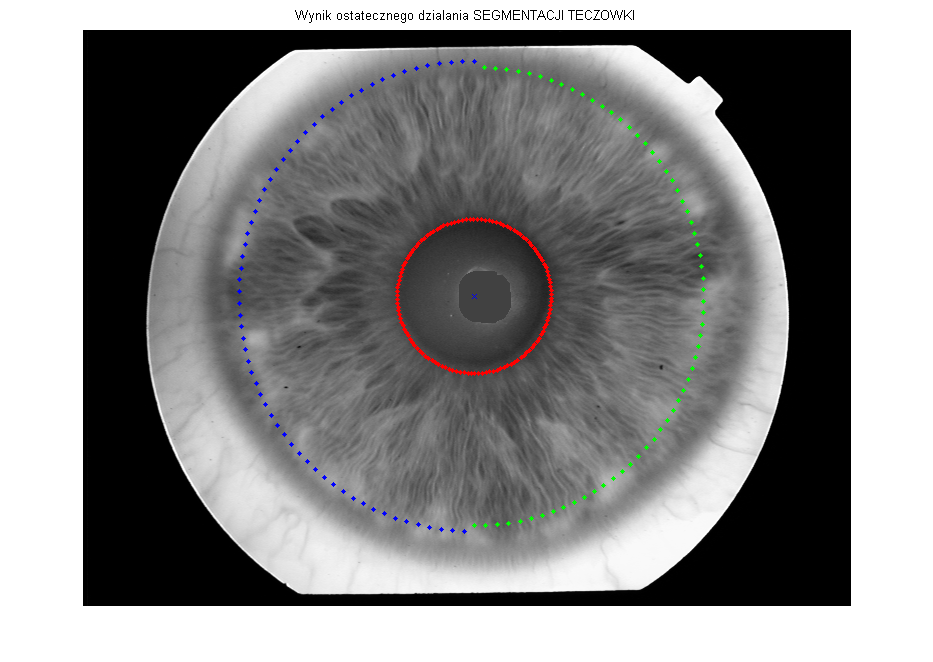
\includegraphics[scale=0.5]{calosc.png}
\caption{Obraz po realizacji algorytmu Daugmana}
\label{fig:przykladDaugman}
\end{center}
\end{figure}

Następnym rozwiązaniem jest metoda Wildes'~a \cite{Wildes}, która jest odmienna od patentu Daugmana. Algorytm ten jest realizowany w~dwóch krokach. Pierwszym jest zamiana oryginalnego obrazu na obraz binarny z~wyznaczonymi krawędziami, które są obecne na obrazie źródłowym. Najczęściej obraz pośredni jest tworzony za pomocą algorytmu Canny'ego. Na zmodyfikowanym obrazie stosowana jest transformacja Hough'~a \cite{KrH11}, dzięki której można znaleźć środek okręgu opisującego tęczówkę oraz jego promień. Wadą tej metody jest trudność ustalenia progu binaryzacji.

Kolejnym sposobem segmentacji tęczówki jest rozwiązanie Camus'a i~Wildes'a \cite{Camus}. Jest to metoda podobna do algorytmu Daugmana, która również polega na wyszukiwaniu tęczówki za pomocą maksymalizacji funkcji. W~tym przypadku funkcją, którą maksymalizujemy jest równanie \ref{eq:camus_wildes} 
\begin{equation}
\label{eq:camus_wildes}
C=\sum_{\theta =1}^{n} ((n-1)\left|\left| g_{\theta,r} \right|\right| - \sum_{\varphi=\theta + 1 } ^{n} \left| \left| g_{\theta,r} - g_{\varphi,r} \right| \right| - \frac{I_{\theta,r}}{n}  )
\end{equation}
gdzie:\\
$ n $ - liczba dyskretnych wartości zmiennej biegunowej $ \theta $, \\
$ g_{\theta, r} $ - pochodna kierunkowa jasności obrazu.

Algorytm ten jest skuteczny głównie w~przypadku, gdzie granica między tęczówką oraz rogówką oraz między tęczówką a~źrenicą jest wyraźna oraz nie ma odblasków lub szumu.

\section{Metody generacji kodu tęczówki}
\label{sec:metodyGeneracjiKodu}

Istnieje wiele metod generacji kodu tęczówki. W patencie Daugmana zastosowano filtrację za pomocą filtrów Gabora \cite{Daugman}, których definicja we współrzędnych biegunowych jest przedstawiona w równaniu \ref{eq:gabor}.
\begin{equation}
\label{eq:gabor}
G(r,\theta) = e^{-2\pi i\omega (\theta - \theta 0)_{e}-(r - r0)2/a2_{e}-(\theta-\theta 0 )2/\beta 2}
\end{equation}
gdzie:\\
$r$ - promień we współrzędnych biegunowych, \\
$\theta$ - kąt w radianach we współrzędnych biegunowych, \\
$ \omega $ - częstotliwość, \\
$ \alpha, \beta $ - stałe.


Wybierane są punkty na obszarze tęczówki, w sposób pozwalający na poprawną analizę w przypadku zmiany jej rozmiaru. Jest to istotna kwestia, ponieważ w zależności od jasności otoczenia zmienia się rozmiar źrenicy, co implikuję zmianę rozmiaru tęczówki. Punkty są następnie filtrowane z~użyciem filtrów Gabora, dla różnych kierunków. W rezultacie otrzymywana jest (dla jednego punktu) liczba zespolona. Następuje kodowanie otrzymanej liczby w następujący sposób: 1, jeśli dana część jest większa od zera lub 0, jeśli jest mniejsza bądź równa zeru. W ten sposób otrzymywany jest bitowy kod (zwykle o~długości 2048 bitów, jest to zależne od liczby wybranych punktów). Przykładowy wybór punktów jest przedstawiony na rysunku \ref{fig:przykladPunkty}

\begin{figure}
\begin{center}
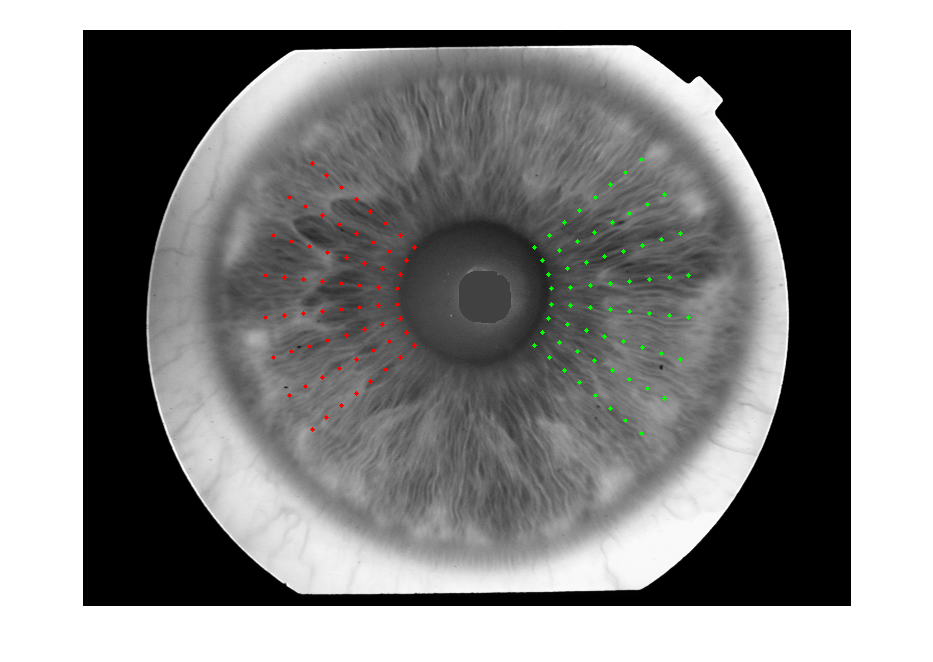
\includegraphics[scale=0.5]{punkty.png}
\caption{Przykładowy wybór punktów}
\label{fig:przykladPunkty}
\end{center}
\end{figure}

Inne podejście stosują Sun i~Tan w swojej pracy \cite{TaSu09}. Proponują użycie tak zwanych \emph{ordinal measures} do rozpoznawania na podstawie tęczówki. Wybiera się w nich dwa obszary, oblicza sumę jasności pikseli w~tych obszarach i~w~zależności od tego, który obszar ma wyższą sumę, koduje się 1 lub 0. Ta metoda jest szybka oraz według twórców wykazuje dobre wyniki.

\section{Metody porównania kodów tęczówek}
\label{sec:metodyPorownaniaKodow}
Główną metodą stosowaną do porównywania kodów tęczówek jest, zaproponowane przez Daugmana, wyznaczanie odległości Hamminga. Odległość Hamminga określa liczbę bitów, których wartości są różne w~dwóch porównywanych kodach. Zaletą tej metody jest szybkość obliczeń oraz prostota implementacji, dlatego została użyta w niniejszej pracy. Inne metody są przedstawione w pracy \cite{Gl11}. Wśród innych metod można wyróżnić bazujące na sieciach neuronowych. Przykładem może być wykorzystanie sieci neuronowych o radialnych funkcjach bazowych lub sieci samoorganizujących się na zasadzie współzawodnictwa przedstawione w pracy \cite{TP11}.
